\setchapterstyle{kao}
\setchapterpreamble[u]{\margintoc}

\chapter{Design and Simulation} % How I thought it was going to work
\labch{tc-design-and-simulation}

\textbf{Disclaimer:} This process was a lot more length and tedious than depicted in the following chapter. It mostly consisted of trial and error, which started with an more or less educated guess and ended in cluelessness and despair. But those errors don't add a lot of value to understanding the topic, so I won't go into much detail.

\section{The Coils}

The goal was to design an air coil with a resonant frequency of 4MHz. This frequency was chosen, since it is high enough to work well with an class E amplifier, but low enough to not run into too many RF related problems. It was also already known to have worked with a few other class E tesla coils.

\subsection{Rough Estimation of the Secondary Coil}

The inductance of a single-layered air solenoid coil can be calculated with

\begin{equation}\label{eq-inductivity}
    L = \mu_0 \frac{N^2 A}{l}
\end{equation}

The parasitic capacitance, depending on its length \(l\) and its diameter \(D\) can be calculated with\sidecite{self-capacitance}

\begin{equation}\label{eq-parasitic-capacitance}
    C_L = \frac{4\varepsilon_0}{\pi} \cdot l \cdot \left( 1 + 0.8249 \frac{D}{l} + 2.329 \left(\frac{D}{l}\right)^{1.5}\right)
\end{equation}

Defining the length to diameter ratio of the coil to be 4, and \(d_w\) to be the diameter of the wire, both formulas can be rewritten to only depend on \(l\) and \(d_w\). 

\begin{equation}
    L = \mu_0 \frac{l^3\ \pi}{32 d_w^2}
\end{equation}

\begin{equation}
    C_L = \frac{4\varepsilon_0}{\pi} \cdot l \cdot 1.49735
\end{equation}

Those equations can then be set into the formula for the resonant frequency of an LC circuit.

\begin{equation}
    f = \frac{1}{2\pi \cdot \sqrt{0.1872 \cdot \dfrac{1}{d_w^2} \cdot \mu_0 \varepsilon_0 \cdot l^4}}
\end{equation}

Rearranging the equation to \(l\)

\begin{equation}
    l = \frac{1}{\sqrt[\scalebox{1}{4}]{4\pi^2 f^2 \cdot0.1872 \cdot \dfrac{1}{d_w^2} \cdot \mu_0 \varepsilon_0}}
\end{equation}

With a frequency of 4MHz and a wire diameter of 0.35mm, the length of the coil turns out to be around 100mm and the diameter therefore around 25mm.

Due to the materials available, a 30 mm tube was used to wind the wire around. By using equation \ref{eq-inductivity} and \ref{eq-parasitic-capacitance}, an equation can be derived, which describes the relationship of all relevant variables.

\begin{equation}
    f = \frac{1}{2\pi \dfrac{D}{d_w} \sqrt{\mu_0 \varepsilon_0 \left( l^2 + 0.8245 D l + 2.329 D^{1.5} \sqrt{l} \right)}}
\end{equation}

Using Wolfram Alpha to solve this equation for \(l\) with a \(D\) of 30 mm gives a length of 112 mm.
% 4000000 = 1/(2π(0.03/0.00035)Sqrt[11.1265e-18*(Power[x,2]+0.8245*0.03*x+2.329*Power[0.03,1.5]*Sqrt[x])]) solve for x

\subsection{Tuning the Secondary Coil}\label{TC-tuningTheSecondary}

Tuning the coil to the correct frequency is essential, because all calculated values from above are highly idealized. For example, equation \ref{eq-parasitic-capacitance} is said to have a standard deviation of \(\sigma_{CL} \text{in pF} = 3.6 \cdot D\), which leads to a standard deviation of around 116 kHz of the resonant frequency of the coil. In addition, the relative permeability and permittivity factor of the carrier material are not taken into consideration in the calculations.

The coil was tuned by exciting the base of the secondary coil with a sinusoidal voltage. An oscilloscope probe, formed into a current loop, was placed near the top of the coil. The closer the excitation frequency was to the resonant frequency of the coil, the higher the measured voltage on the oscilloscope. The frequency, at which the measured voltage was at its maximum, was the resonant frequency of the coil. By adding or removing windings, the resonant frequency could be lowered or raised, until it exactly matched 4MHz\sidenote{In order to avoid adding windings, which is more tedious than removing them, the coil was wound a little longer than calculated}. % Add how close the original calculations were

\subsection{Designing the Primary Coil}
\label{sec:designing-the-primary}

The primary coil offers a lot of design freedom and flexibility, but this also means, that there is no \enquote{correct} or \enquote{ideal} design, but only one, which has been observed to work well. It mostly comes down to optimizing the coupling coefficient between the two coils. If it's too low, not enough energy will be transferred to the secondary, but to raise it, the coils have to be moved closer together which leads to flashover, due to too low insulation. % Test tesla coil with coupling factor of 0.10 to 0.15  Source: book page 55
This limitation can be bypassed by making the primary coil smaller at the bottom, where the voltage is higher and larger at the top, where the voltage is higher. This results in the well-known conical shape known from many tesla coils.

\begin{marginfigure}
\centering
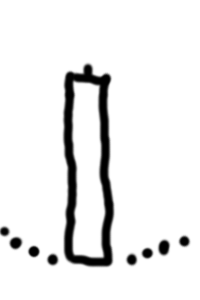
\includegraphics[width=0.6\textwidth]{simon/resources/teslaCoilSketch.png}
\end{marginfigure}

\subsection{Simulating the Coupling Coefficient}

In order to simulate the resonant transformer, its coupling coefficient has to be known. It describes how tightly the two coils are magnetically coupled and how much of the generated magnetic field of one coil is induced in the other. The simulation tool EleFAnT2D\sidenote{\textbf{Ele}ctromagnetic \textbf{F}ield \textbf{An}alyis \textbf{T}ool, developed IGTE, TU Graz} was used to simulate the magnetic flux in the system. The coupling coefficient can be described as

\begin{equation}
    k = \frac{\Phi_{ind}}{\sqrt{\Phi_P \cdot \Phi_S}}
\end{equation}

where \(\Phi_{ind}\) is the flux linkage between the two coils and \(\Phi_P\) and \(\Phi_S\) are the flux of the primary and secondary coil, respectively.\todo{Is it really?} By using this formula and the simulated values, the coupling factor as a function of the vertical displacement of the primary coil has been calculated as can be seen in figure \ref{fig:coupling-factor}.

\begin{figure}[h!]
    \centering
    \begin{tikzpicture}
    \begin{axis}[
    width = 0.9\textwidth,
    minor tick num = 1,
    grid = both,
    ymax = 25,
    xmin = -20,
    xmax = 20,
    xlabel = Vertical displacement in mm,
    ylabel = Coupling factor in \%
    ]
    \addplot+[mark options={black!50}, draw=black] table [x=d, y=k, col sep=comma]{simon/resources/couplingFactor.csv};
    \draw (axis cs:0,-10) -- (axis cs:0,18.397) -- (axis cs:-20,18.397);
    \draw (axis cs:-18,18.9) node(){\(18.4\)};
    \end{axis}
    \end{tikzpicture}
    \caption{Position dependent coupling factor}
    \label{fig:coupling-factor}
\end{figure}

As expected, the coupling factor gets smaller the farther away the primary coil moves from the middle of the secondary coil.

\section{The Class-E Stage}

As already explained in aaaaa, it is everything but trivial to design a class E amplifier to drive a tesla resonator. However, for the sake of demonstration, the following subsection will go through the design process of a class E amplifier with an ohmic load.

\subsection{The Design Process}

Nathan Sokal, who popularized the class-E amplifier along with Alan Sokal, presented a set of design equations in 2001 \sidecite{sokal-qex}. Unlike previously published equations, they include the dependence of the loaded Q factor\sidenote{It describes how damped a resonator is, or in other words, how quickly it dissipates its oscillating energy.} as well as on the output power.

The goal of this amplifier is to create 50W of output power with a load of 22\(\Omega\) at a frequency of 4MHz. The Q factor of the load will be assumed as 5, since this is a common starting value. The switching device will be a MOSFET, so the saturation voltage used in the equations can be set to zero. The necessary supply voltage can then be calculated as

\begin{equation*}
    V_{CC} = \sqrt{R \cdot P \cdot 1.7337 \cdot \frac{1}{1.001245 - \frac{0.451759}{Q_L} - \frac{0.402444}{Q_L^2}}}\textnormal{ ,}
\end{equation*}

which turns out to be 46.17V. The expected peak drain-source voltage on the MOSFET is 3.56 times the supply voltage plus a safety factor of around 20\%, which means that the MOSFET has to have a drain-source breakdown voltage of at least 197V. By assuming \(L_1\) to be 130\(\mu\)H, \(C_1\), \(C_2\), and \(L_2\) can be calculated with

\begin{equation*}
    C_1 = \frac{1}{34.2\cdot f R} \cdot \left( 1 + \frac{0.914}{Q_L} - \frac{1.03}{Q_L^2} \right) + \frac{0.6}{(2 \pi f)^2  \cdot L_1} = 387 pF\textnormal{ ,}
\end{equation*}

\begin{equation*}
    C_2 = \frac{1}{2 \pi  f  R} \cdot \frac{1}{Q_L - 0.105} \cdot \left( 1 + \frac{1.01}{Q_L - 1.79} \right) - \frac{0.2}{(2 \pi f)^2 \cdot L_1} = 482pF \textnormal{ , and}
\end{equation*}

\begin{equation*}
    L_2 = \frac{Q_L \cdot R}{2 \pi f} = 4.38\mu H\textnormal{ .}
\end{equation*}
    
As recommended in \sidecite{sokal-qex}, the impedance \(X_{L1}\) is at least 30 times greater than the impedance \(X_{C1}\) at the operating frequency. The value for \(C_1\) actually is the sum of the component \(C_1\) and the MOSFET's output capacitance. This means that the MOSFET has to have

\begin{itemize}
    \item a drain-source breakdown voltage greater than 197V,
    \item an output capacitance less than 387pF,
    \item switching times much smaller than 250ns, and
    \item a maximum power dissipation of at least 5W.
\end{itemize}

One MOSFET which meets all these criteria is the BSC12DN20. It has a drain-source breakdown voltage of 200V, an output capacitance of 39pF, turn-off and turn-on times of less than 5 ns and a maximum power dissipation of 50W.
    
\section{The Interrupter}

\subsection{Fiber Optic Receiver}

\subsection{MOSFET protection circuit}

Directly applying the interrupting technique to the class E circuit by just turning it on and off at any given moment would violate both the \gls{zvs} and \gls{zcs} conditions. In the worst case, switching the MOSFET on when the voltage is at its maximum and turning it off when the current is at its maximum a few thousand times a second would result in huge switching losses and device failure. Therefore a security mechanism has to be implemented.

One solution is to sample the interrupter signal and only apply it on every falling edge of the 4MHz base signal. The sampling could be done with a falling-edge triggered D-type flip-flop, whose output gets fed into an AND gate along with the base signal.

\begin{figure}[h!]
    \centering
    \caption{Bottom side text}
    \begin{circuitikz}[european]
      \draw (0,0) node[flipflop, flipflop def = {t1 = D, c3 = 1, n3 = 1, t3 = CLK, t6 = Q}](D){};
      \draw (4,.61) node[and port](A){};
      \draw (D.pin 6) -- (A.bin 1);
      \draw (D.pin 1) node[left]{INT};
      \draw (D.pin 3) ++(-.5,0) node[left]{4MHz} -- (D.pin 3);
      \draw (D.pin 3) ++(-.25,0) to[short, *-] ++(0,-.8) -- ++(3,0) node(n1){} -- (n1 |- A.bin 2) -- (A.bin 2);
      \draw (A.bout) ++(.4,0) node[right]{OUT};
    \end{circuitikz}
    \phantom{a}
    \vspace{10mm}
    \phantom{a}
    \begin{tikztimingtable}[timing/xunit = 5mm, timing/slope = 0.05]
      4MHz & 3{2{l}2{h}} N(a) 4{2{l}2{h}} N(b) 2{2{l}2{h}} \\
      INT  & 11{h} 16{l} 9{h} \\
      Q    & 12{h}16{l} 8{h} \\
      OUT  & 3{2{l}2{h}}16{l}2{2{l}2{h}} \\
      \extracode
      \draw[dotted, darkgray] (a) -- ++(0,-6);
      \draw[dotted, darkgray] (b) -- ++(0,-7);
    \end{tikztimingtable}
\end{figure}